\tikzstyle{block} = [rectangle, draw, 
    text width=8em, text centered, rounded corners, minimum height=4em]
    
\tikzstyle{line} = [draw, -latex]

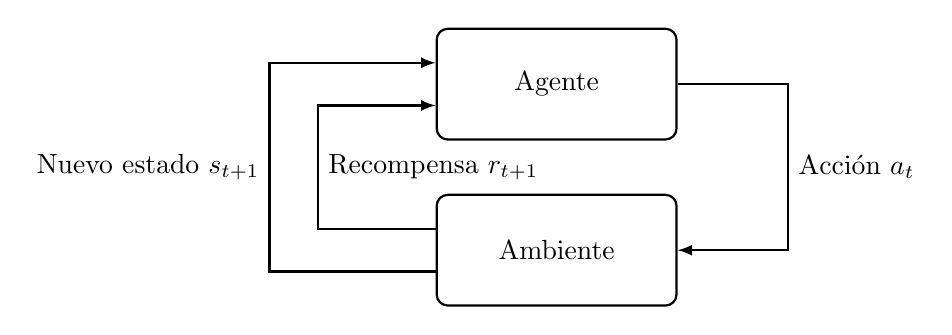
\begin{tikzpicture}[node distance = 6em, auto, thick]
    \node [block] (Agent) {Agente};
    \node [block, below of=Agent] (Environment) {Ambiente};
    
     \path [line] (Agent.0) --++ (4em,0em) |- node [near start]{Acción $a_t$} (Environment.0);
     \path [line] (Environment.190) --++ (-6em,0em) |- node [near start] {Nuevo estado  $s_{t+1}$} (Agent.170);
     \path [line] (Environment.170) --++ (-4.25em,0em) |- node [near start, right] {Recompensa $r_{t+1}$} (Agent.190);
\end{tikzpicture}